\documentclass[11pt, oneside]{article} 
\usepackage{geometry}
\geometry{letterpaper} 
\usepackage{graphicx}
	
\usepackage{amssymb}
\usepackage{amsmath}
\usepackage{parskip}
\usepackage{color}
\usepackage{hyperref}

\graphicspath{{/Users/telliott_admin/Tex/png/}}
% \begin{center} 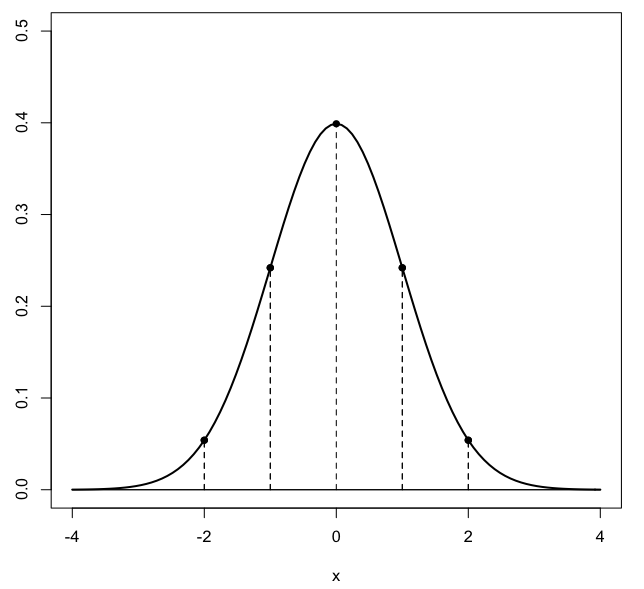
\includegraphics [scale=0.4] {gauss3.png} \end{center}

%break
\title{Euler 3D rotation}
\date{}

\begin{document}
\maketitle
\Large

More than once, we have derived the matrix equations for rotation in two dimensions.  For a ccw rotation
\[
\begin{bmatrix}  
\cos \theta  & -\sin \theta \\  
\sin \theta & \ \ \cos \theta  
\end{bmatrix}
\begin{bmatrix}  
x  \\  
y  
\end{bmatrix}
=
\begin{bmatrix}  
x \cos \theta - y \sin \theta  \\  
x \sin \theta + y \cos \theta 
\end{bmatrix}
\]
So for $\theta = \pi/2$ we have $\cos \theta = 0$ and $\sin \theta = 1$ and then 
\[
\begin{bmatrix}  
0  & -1 \\  
1 & \ \ 0  
\end{bmatrix}
\begin{bmatrix}  
x  \\  
y  
\end{bmatrix}
=
\begin{bmatrix}  
- y  \\  
 \ \  x
\end{bmatrix}
\]


In three dimensions, it gets a lot trickier.  But one way to think about it is to imagine three sequential rotations about the $x$, $y$, and $z$-axes.  Any particular rotation can be accomplished in this way.  And by matrix multiplication, we can generate a single $R$ matrix for the composed rotation.

The corresponding $R$ matrices are
\[
R_x =
\begin{bmatrix}  
1 & 0 & 0 \\  
0 & \cos \theta  & -\sin \theta \\  
0 & \sin \theta & \ \  \cos \theta
\end{bmatrix}
\]
\[
R_y = 
\begin{bmatrix}  
\ \ \cos \theta & 0 & \sin \theta \\  
0 & 1  & 0 \\  
-\sin \theta & 0 & \cos \theta
\end{bmatrix}
\]
\[
R_z =
\begin{bmatrix}  
\cos \theta  & -\sin \theta & 0 \\  
\sin \theta & \ \  \cos \theta  & 0 \\  
0 & 0 & 1
\end{bmatrix}
\]
or, re-writing them to distinguish the three angles involved
\[
\begin{bmatrix}  
1 & 0 & 0 \\  
0 & \cos \alpha  & -\sin \alpha \\  
0 & \sin \alpha & \ \  \cos \alpha
\end{bmatrix}
 \ \ \
\begin{bmatrix}  
\ \ \cos \beta & 0 & \sin \beta \\  
0 & 1  & 0 \\  
-\sin \beta & 0 & \cos \beta
\end{bmatrix}
 \ \ \
\begin{bmatrix}  
\cos \gamma  & -\sin \gamma & 0 \\  
\sin \gamma & \ \  \cos \gamma  & 0 \\  
0 & 0 & 1
\end{bmatrix}
\]
It matters which order we do things in, because in general $AB \ne BA$ in matrix multiplication.  The multiplication is a bit of a mess.

Euler's special insight is to realize that \emph{any} such rotation leaves two points on a sphere unchanged, so that it corresponds to a single rotation around a particular axis.  His proof is a geometric proof.

The idea that two points are fixed, so the sphere just rotates, can be restated in the language of linear algebra.  We say that the vector $\mathbf{v}$ is an eigenvector of the rotation matrix $R$, with eigenvalue $1$.
\[ R \mathbf{v} = \mathbf{v} \]

The special vector $\mathbf{v}$ connects the two points that don't rotate, hence it does not change either.  After $R$ operates on $\mathbf{v}$, $\mathbf{v}$ is unchanged. 

There is a proof that such an eigenvector $\mathbf{v}$ exists, that is presented in the wikipedia article, and I would like to try to follow it here.

As a preliminary, the proof states that a fundamental property of rotation matrices is that the transpose is equal to the inverse:
\[ R^T R = R R^T = I \]

We can certainly see that is true  for 
\[ R_{ccw} = 
\begin{bmatrix}  
\cos \theta  & -\sin \theta \\  
\sin \theta & \ \ \cos \theta  
\end{bmatrix}
\]
because constructing the inverse rotation $R_{cw}$ (undoing $R_{ccw}$ so that $R_{ccw} R_{cw} = I$), amounts to substituting $-\theta$ for $\theta$, which changes the sign of the sine terms but does nothing to the cosine.  

A similar thing happens for the 3D versions, where the sine terms have opposite sign and are symmetric, switching places in the transpose, while the cosine terms do not change sign and are on the diagonal.

Furthermore, it is clear that the determinants of $R$ and $R^T$ are equal
\[ | R^T| = |R| \]
because (as before) the transpose just switches the sign of the sine terms.  (Actually, in the previous write-up we showed that this is true for any square matrix).  Also, we can see that these properties are true for any rotation in $2D$, since for any such rotation, we must be able to specify a corresponding angle $\theta$ through which to turn to reach that orientation.

It's not quite so clear that the same thing can be said for any rotation matrix in 3D obtained by sequential application of $R_x$, $R_y$ and $R_z$, but it's true.  

Multiplying out 
xxxx

Using the property that $R^T = R^{-1}$ 
\[ |R^T R| = |R^{-1} R| =  |I| = 1 \]
and since $|AB| = |A| |B|$ (the product rule)
\[ 1 = |R^T R| = |R^T| |R| \]
but above we said that $|R^T| = |R|$ so
\[ 1 = |R|^2 \]
which implies that
\[ |R| = \pm 1 \]

Note:  we proved that $|AB| = |A| |B|$ following an argument from Strang, in another write-up.

If the determinant is $1$, the rotation is called a proper rotation, while if it is $-1$, the rotation is an \emph{improper} rotation, consisting of a reflection plus a rotation.  Our rotation matrices have $|R| = 1$ and so 
\[ 1 = |R^T R| = |R^T| |R| = |R^T| \]

You should know about  eigenvalues for the following argument to make sense.  If the matrix $R$ has an eigenvalue $\mathbf{v}$ with eigenvalue $\lambda = 1$
\[ R \mathbf{v} = \mathbf{v} \]
The vector $\mathbf{v}$ is unchanged by the rotation.
Thus 
\[ R \mathbf{v} - \mathbf{v} = 0 \]
\[ = (R - I) \mathbf{v} = 0 \]
which has non-zero vector solutions solutions only if the determinant of $R-I$ is equal to zero
\[ |R - I | = 0 \]
which is the same thing as saying that $\lambda = 1$ is at least one eigenvalue of the rotation matrix $R$, so there is an eigenvector that is unchanged under rotation.

So far we have that
\[ |R| = |R^T| = 1 \]

Our argument goes like this:

(1) Since $|R| = |R^T|$, and since it is only the values on the diagonal which change (decreasing by $1$) when doing the subtraction $R-I$, and furthermore, the transpose does not alter the values on the diagonal:
\[ |R-I| = |R^T - I| \]

(2) Since $R^T = R^{-1}$
\[ = |R^{-1} - I| \]

The following is a matrix identity
\[ A(B-C) = AB - AC \] 
It can be proved by following the components of the vectors, but it really follows from the distributivity of the dot product where
\[ \mathbf{a} \cdot (\mathbf{b} - \mathbf{c}) = \mathbf{a} \cdot \mathbf{b} - \mathbf{a} \cdot \mathbf{c} \]
and since each entry of all the products is in this form:
\[ AB_{mn} = \mathbf{a}_{mi} \cdot \mathbf{b}_{jn} \]
(All the entries from row $m$ times the entries from column $n$.)
It works.

(3) Using $A(B-C) = AB - AC$, we can go in reverse to rearrange the above to
\[ |R^{-1} - I| = |-R^{-1}(R - I)| \]
(switching the order of terms and using $R^{-1} R = I$.

(4) But again $|AB| = |A| |B|$ so
\[ = |-R^{-1} | |R-I| \]
(5) And $ | -R^{-1}| = -| R^{-1} | $ by the basic properties of determinants, but $|R^{-1}| = 1$ so
\[ = - | R-I | \]
Summarizing, we have shown that
\[ |R-I| = - |R-I| \]

Since the thing itself $|R-I|$ is equal to its negative, it must be that $|R-I| = 0$, which completes the proof.
\end{document}  